\section{Experiments}
\label{sec:experiments}

\subsection{Dataset and Protocol}

MFNet contains 784 aligned RGB-thermal training pairs and 392 test pairs captured in
urban driving scenes during day and night \cite{ha2017mfnet}. We use the eight
foreground classes plus the unlabeled class, report the official nine-class mIoU used
by the training code, and additionally report foreground mIoU and nighttime pedestrian
IoU. The nighttime subset is defined by the ``N'' prefix in the MFNet filenames, the
same convention used by the benchmark. All models use the CMNeXt-B2 backbone with a
SegFormer-B2 initialization \cite{xie2021segformer,zhang2023delivering}, a batch size of
eight, AdamW with a learning rate of $6\times10^{-5}$, and 120 epochs. The RGB-only and
thermal-only experts are trained with the same schedule and augmentation; the only
difference is the input modality and, for the thermal expert, the resolution of the
thermal stream.

Low-resolution thermal is simulated by a bicubic round trip, as described in
Section~3.1. We evaluate three budgets: $60\times80$ (\lr{8}, $1/64$ of the RGB
pixels), $120\times160$ (\lr{4}, $1/16$), and $240\times320$ (\lr{2}, $1/4$). The
full-resolution teacher is a two-stream CMNeXt-B2 trained on the full thermal stream;
we use it only as a reference for the recovery calculation and do not place it in the
main table, because its schedule is longer than the 120-epoch experts.

\subsection{How Many Thermal Pixels Are Needed?}

Table~\ref{tab:budget} and Figure~\ref{fig:pareto} summarize the budget sweep. The
thermal-only model improves monotonically on nighttime pedestrians as the budget grows:
58.48 IoU at $60\times80$, 61.88 at $120\times160$, and 62.48 at $240\times320$. The
corresponding recovery of the full-resolution teacher's nighttime advantage is 64\%,
81\%, and 84\%. The knee is therefore at $120\times160$: doubling the linear resolution
from $60\times80$ buys 17 points of recovery, while doubling it again buys only three.
At the same time, overall thermal-only mIoU does not improve with resolution
(55.83, 55.80, 55.24), because the thermal stream loses to RGB on the eight non-person
classes regardless of budget. The budget curve is a statement about the safety class,
not about overall parsing.

\begin{table}[t]
\centering
\caption{Thermal sensor budget on MFNet (392-image official test). Gate rows are mean
$\pm$ standard deviation over three gate-training seeds with frozen experts. Thermal
pixels are relative to the $480\times640$ RGB frame.}
\label{tab:budget}
\begin{tabular}{lcccc}
\toprule
Method & thermal pixels & official & fg & night person \\
\midrule
RGB-only (CE120) & 0 & 56.38 & 51.28 & 45.24 \\
Thermal-only \lr{8} & $1/64$ & 55.83 & 50.66 & 58.48 \\
Thermal-only \lr{4} & $1/16$ & 55.80 & 50.62 & 61.88 \\
Thermal-only \lr{2} & $1/4$ & 55.24 & 50.00 & 62.48 \\
\midrule
Gate \lr{8} & $1/64$ & $57.38\pm0.04$ & $52.40\pm0.04$ & $58.46\pm0.14$ \\
Gate \lr{4} & $1/16$ & $\mathbf{57.57\pm0.08}$ & $\mathbf{52.61\pm0.08}$ & $61.36\pm0.39$ \\
Gate \lr{2} & $1/4$ & 57.45 & 52.47 & 61.01 \\
\bottomrule
\end{tabular}
\end{table}

\begin{figure}[t]
\centering
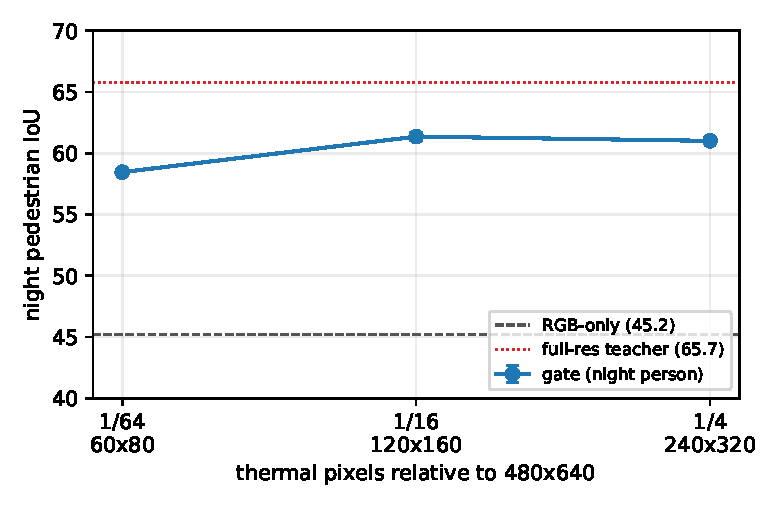
\includegraphics[width=\linewidth]{figures/pareto_night_person.pdf}
\caption{Nighttime pedestrian IoU as a function of the thermal pixel budget. The
thermal expert improves until $120\times160$; the gate adds overall mIoU without
changing the knee. The full-resolution teacher is shown as a reference.}
\label{fig:pareto}
\end{figure}

\subsection{The Gate Makes the Budget Usable}

Table~\ref{tab:budget} also reports the gate. At $120\times160$ the gate reaches
$57.57\pm0.08$ official mIoU and $61.36\pm0.39$ nighttime pedestrian IoU, against
56.38 and 45.24 for RGB-only and 55.80 and 61.88 for the thermal expert. The gate
therefore improves overall mIoU by 1.19 and nighttime pedestrian IoU by 16.1 over RGB,
while giving up only 0.5 nighttime pedestrian IoU relative to the thermal expert. The
latter trade is deliberate: the thermal expert is better on pedestrians but worse on
the other classes, and the gate recovers overall parsing without surrendering the
safety gain. At $60\times80$ the gate is $57.38\pm0.04$ and $58.46\pm0.14$; at
$240\times320$ it is 57.45 and 61.01. The knee is stable across budgets, and the
$120\times160$ operating point is the best overall compromise.

Table~\ref{tab:variants} isolates the deployment variants. The full gate, which may
override RGB wherever the experts disagree, reaches 56.20 overall but only 61.17
nighttime pedestrian IoU. The person-constrained gate reaches 57.53 overall and 61.17
nighttime pedestrian IoU, a gain of 1.33 overall over the full gate at the same
pedestrian score. Restricting overrides to the thermal expert's pedestrian prediction
(\texttt{person\_b}) or to a pedestrian probability threshold
(\texttt{person\_prob}) is worse, 57.30 and 57.28 overall, because the RGB expert
sometimes predicts the pedestrian correctly and should not be overridden. The
person-or rule is the only variant that preserves both experts' pedestrian evidence.

\begin{table}[t]
\centering
\caption{Gate variants at $120\times160$ (seed 3407, frozen experts). A is RGB-only,
B is thermal-only; all other rows are gate deployments.}
\label{tab:variants}
\begin{tabular}{lccc}
\toprule
Variant & official & fg & night person \\
\midrule
A (RGB) & 56.38 & 51.28 & 45.24 \\
B (thermal) & 55.80 & 50.62 & 61.88 \\
Full gate & 56.20 & 51.07 & 61.17 \\
Person-or & \textbf{57.53} & \textbf{52.56} & 61.17 \\
Person-B & 57.30 & 52.31 & 58.92 \\
Person-prob & 57.28 & 52.28 & 58.49 \\
\bottomrule
\end{tabular}
\end{table}

\subsection{Where the Gain Comes From}

Figure~\ref{fig:perclass} shows the per-class change from RGB to the person-or gate.
The entire gain is the pedestrian class: $+9.45$ IoU, from 55.79 to 65.24. All other
classes change by at most 0.37 IoU, and six of the eight change by less than 0.2. This
is the intended behavior of a structural safety prior: it repairs the class that
motivates the thermal sensor and leaves the rest of the scene to the higher-resolution
RGB expert. A global fusion model cannot make this separation, which is why its
overall mIoU is below RGB-only despite a much stronger pedestrian score.

\begin{figure}[t]
\centering
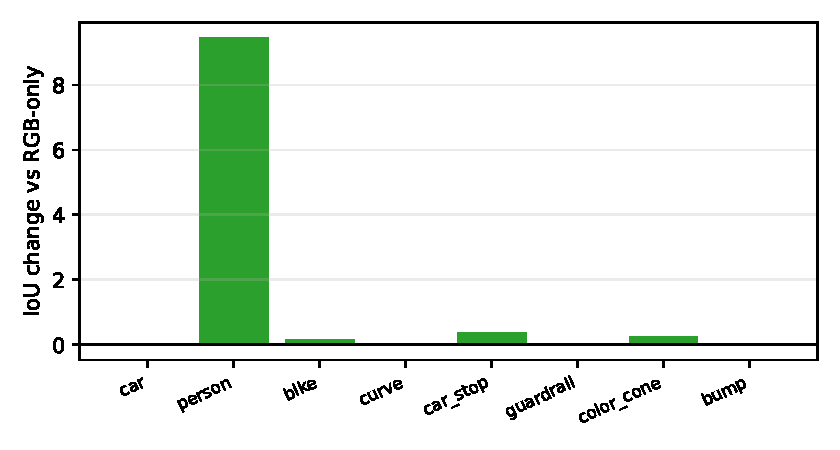
\includegraphics[width=\linewidth]{figures/per_class_delta.pdf}
\caption{Per-class IoU change from RGB-only to the person-or gate at
$120\times160$. The gain is concentrated in the pedestrian class.}
\label{fig:perclass}
\end{figure}

\subsection{Robustness to Corrupted RGB}

We corrupt RGB at test time with the same hard-condition family used for gate training:
a contrast reduction to 0.55, Gaussian noise, and an optional average blur. The thermal
stream is left at its budget. Table~\ref{tab:degraded} and
Figure~\ref{fig:degraded} report the result. RGB-only collapses from 56.38 to 47.95
official mIoU and from 45.24 to 32.74 nighttime pedestrian IoU. The thermal expert
improves to 50.70 and 62.02, because it is unaffected by the RGB corruption. The full
gate reaches 51.10 overall and 60.95 nighttime pedestrian IoU, the best overall result
under corruption. The person-or gate reaches 49.49 and 60.95: its fixed constraint
prevents it from using thermal evidence on non-person classes that RGB can no longer
parse, which is the expected cost of the safety prior. The clean/degraded trade-off is
the honest limitation of a fixed constraint; an image-quality-conditioned gate is
future work.

\begin{table}[t]
\centering
\caption{Clean versus corrupted RGB at $120\times160$. Corruption is applied only to
RGB; thermal is unchanged. Official mIoU / nighttime pedestrian IoU.}
\label{tab:degraded}
\begin{tabular}{lcccc}
\toprule
 & \multicolumn{2}{c}{clean} & \multicolumn{2}{c}{corrupted} \\
\cmidrule(lr){2-3}\cmidrule(lr){4-5}
Method & official & night person & official & night person \\
\midrule
RGB-only & 56.38 & 45.24 & 47.95 & 32.74 \\
Thermal-only & 55.80 & 61.88 & 50.70 & 62.02 \\
Full gate & 56.20 & 61.17 & \textbf{51.10} & 60.95 \\
Person-or & \textbf{57.53} & 61.17 & 49.49 & 60.95 \\
\bottomrule
\end{tabular}
\end{table}

\begin{figure}[t]
\centering
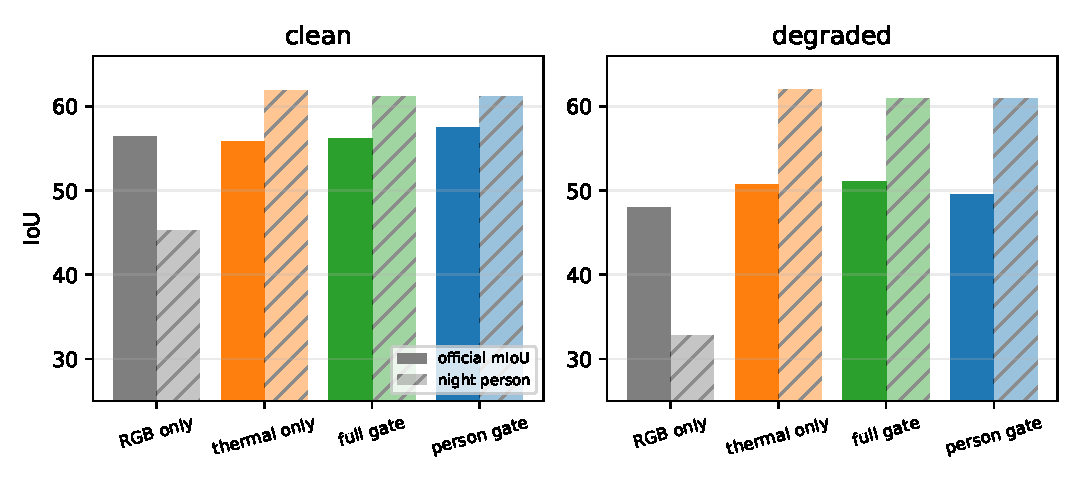
\includegraphics[width=\linewidth]{figures/clean_degraded.pdf}
\caption{Clean versus corrupted RGB. The full gate is the best overall model under
corruption; the person-or gate is the best clean model.}
\label{fig:degraded}
\end{figure}

\subsection{Ablations and Cost}

Hard-condition augmentation is neutral on clean data and useful under corruption.
With augmentation, the full gate reaches 56.20 clean and 51.10 corrupted; without it,
55.63 and 50.23. The gain is +0.57 clean and +0.87 corrupted. For the person-or gate
the clean difference is negligible (57.53 versus 57.54), so the augmentation is not
tuning the clean score; it is buying robustness. The class-gate baseline, which selects
one expert per class on training accuracy, collapses to the thermal expert on all nine
classes and reaches only 55.80 official mIoU, below RGB-only. This is the negative
result that motivates the spatial gate and the held-out selection protocol.

The compute cost is measured on an RTX 4090 at $480\times640$ with batch size one. The
RGB expert has 25.8M parameters, 46.2 GFLOPs, and 11.0 ms latency. The thermal expert
has 58.7M parameters, 74.3 GFLOPs, and 29.8 ms. The gate has 1.9M parameters, 45.6
GFLOPs, and 3.3 ms. The joint system has 86.4M parameters, 166.0 GFLOPs, and 42.6 ms,
2.6 times the RGB-only latency. The contribution is a sensor-pixel budget, not a
compute budget; a native low-resolution thermal branch or a single-model distillation
of the gate would reduce the compute, and we leave both to future work.
